%
% File acl2018.tex
%
%% Based on the style files for ACL-2017, with some changes, which were, in turn,
%% Based on the style files for ACL-2015, with some improvements
%%  taken from the NAACL-2016 style
%% Based on the style files for ACL-2014, which were, in turn,
%% based on ACL-2013, ACL-2012, ACL-2011, ACL-2010, ACL-IJCNLP-2009,
%% EACL-2009, IJCNLP-2008...
%% Based on the style files for EACL 2006 by 
%%e.agirre@ehu.es or Sergi.Balari@uab.es
%% and that of ACL 08 by Joakim Nivre and Noah Smith

\documentclass[11pt,a4paper]{article}
\usepackage[hyperref]{vocabbysty}

\usepackage{times}
\usepackage{latexsym}
\usepackage{graphicx}
\usepackage{subfig}
\usepackage[most]{tcolorbox}
\usepackage{lipsum}
\usepackage{hyperref}

\renewcommand{\arraystretch}{1.75}
\setlength{\arrayrulewidth}{1mm}
\setlength{\tabcolsep}{18pt}
\graphicspath{ {./images/} }
\aclfinalcopy % Uncomment this line for the final submission
\def\aclpaperid{***} %  Enter the acl Paper ID here

%\setlength\titlebox{5cm}
% You can expand the titlebox if you need extra space
% to show all the authors. Please do not make the titlebox
% smaller than 5cm (the original size); we will check this
% in the camera-ready version and ask you to change it back.

\newcommand\BibTeX{B{\sc ib}\TeX}

\title{Structured vocabulary learning within the context of learner's domain}
\author{Haemanth Santhi Ponnusamy \qquad Himanshu Bansal \\
  International Studies of Computational Linguistics(ISCL) \\
  Eberhard Karls Universität Tübingen, 
  Germany \\ \tt \small \{haemanth.santhi-ponnusamy,himanshu.bansal\}@student.uni-tuebingen.de}

\date{}

\begin{document}
\maketitle
\begin{abstract}
 This work is a proposal for a customised vocabulary learning application, which is designed for intermediate language learners who are bored with the traditional approaches that are generalised for learners of a wide variety. This application provides an option for the learners to choose the text of their interest, from which it automatically builds a structure of the underlying vocabulary and the content for vocabulary learning. Based on the interactions with the learner, the application dynamically tweaks the difficulty of the activities to achieve maximised gain. This application is observed to build a meaningful structure of the vocabulary which efficiently helps in reducing the number interactions required to cover the entire vocabulary.
\end{abstract}

\section{Introduction}

Vocabulary learning is an open-ended task as the languages are vast and still
evolving with the addition of new words now and then. Which makes it hard for the vocabulary learners to sense the progress. Popular vocabulary learning applications such as \textit{Duolingo} \footnote{\url{https://www.duolingo.com/}}, \textit{Memrise}\footnote{\url{https://www.memrise.com/}}, \textit{LingoDeer}\footnote{\url{https://www.lingodeer.com/}}, \textit{Drops}\footnote{\url{https://languagedrops.com/}} starts from very basic words of the language. Which are suitable for the beginners, but not for our target learners. They might want to start at an intermediate level. 

Though the application like \textit{Vocabulary.com}\footnote{\url{https://www.vocabulary.com/}} allows the learner to choose the selected set of words they want to learn and applications like \textit{busuu}\footnote{\url{https://www.busuu.com/}} enables the learner to choose the level competency at which they want to learn words. Still, they do not allow them to choose the context in which they want to learn them. Even an adaptive system that tries to adapt to the learner needs lots of interactions to get a sense of learner's vocabulary knowledge.

Another major issue of these tools is the quality of example sentences used as context. They are mostly very generic and sometimes unnatural. This nature is because those applications are designed to support learners with a wide range of language competence, background, area of interest, learning goals. Also, it is hard for developers to manually create contents aligned with different domain to satisfy all kind of learners.

In this paper, we propose an approach to overcome the above-mentioned
difficulties in building an application that could potentially satisfy our targeted
learners. We do this by partially sharing the problem with the learner to choose the text of their interest and reading level. Then we process the selected text to build a network of candidates to efficiently model the limited language space and generate useful activities from them. This helps the learner in defining the sub-space of the language to master. By this way, one could choose to learn words used in a specific domain with a specific context. So the open-ended problem of learning vocabulary of an entire language can be reduced down to a smaller and self-defined milestone.

\section{Related works}
There are many vocabulary learning tools available in the market.
We have gone through many of them to compare the advantages and disadvantages of each.
The study by ~\cite{chen2008personalised} presents a personalised mobile application for
learning English vocabulary based on learning memory cycle and item response theory, which helps in selecting appropriate vocabulary according to the individual.
After that, this group also presented another paper for English vocabulary
learning by creating a mobile application which notifies the user about current
English news but according to the reading abilities of the user. Which they found out
by using fuzzy item response theory. This application helps in improving English reading ability to users.
In the paper presented by ~\citet{wong2010mobile}, In learning English prepositions and Chinese idioms, respectively,
the primary school students used the mobile devices assigned to them on a one-to-one basis
to take photos in real-life contexts to construct sentences with the newly acquired prepositions or idioms.

We have gone through a lot of methods for graph creation for vocabulary generation as
it is the most important step of vocabulary learning. Yo ~\citet{ehara2014formalizing}
from National Institute of Information and Communications Technology, Tokyo proposed
a method by formalising heuristic techniques as a graph-based non-interactive active
learning method as applied to a special graph. They showed that by extending the graph,
they could retrieve additional functionality such as incorporating domain specificity and sampling from multiple corpora.
~\citet{zhang2001learning} proposed a method in which they used a machine-learning based approach
that can be trained for different domains and requires almost no manual rules.
They adopted a dependency grammar link for this model.

But in any of research learner is not able to learn vocabulary from the uploaded text. This is the problem that we overcome in our system so that learner can use own text
according to the level of knowledge or interest. This type of system also helps to prevent predefined selected vocabulary by developers.  

\section{Building vocabulary}
One of the key features of our application is to allow learners to choose their preferred text for learning vocabulary. This provides the freedom to choose the context in which they enjoy learning and to choose a subspace of the language, which they desire to master instead of approaching it as an open-ended problem. The text uploaded should be a plain text (\textit{.txt}), which contains no formatting, only line breaks and spacing. This raw input text is further structured into a meaningful form as described in upcoming sections. We recommend the text to be longer, as we use statistical features (which are discussed in the later sections) to structure the learner text. Thus the quality of structured data is directly proportional to the size of the learner text.

The process of building the vocabulary is independent of the learner. We focus on capturing the underlying vocabulary structure of the text. Each learner text input is a book entry, and all the processed books are stored as a '\textit{library}'. So any new learner can pick a pre-processed book from the library. This feature could also help us to compare and contrast the progression of learning of learners from different background in future.

\subsection{Candidates}

Given that these learners already know some basics of the language, we could eliminate the stop words (commonly used words)\footnote{\url{https://github.com/explosion/spaCy/blob/master/spacy/lang/en/stop_words.py}} that includes the most frequently used words and functional words (the, of, in, on etc.). Another usually eliminated significant category is rare/less frequent words. We remove the words with a frequency of less than five as we need to have a variety of shreds of evidence to generate better activity, which is discussed in \autoref{sec:activity}. 
This elimination also includes the improperly extracted words introduced due to the unregulated learner input structure.

\subsection{Disambiguation}
The candidate words extracted for learning could contain homographs, the set of words that are spelt the same but have a different meaning. An initial step toward disambiguation of the candidate word could be using parts of speech tags ~\cite{wilks1998grammar}. The same words that occur in different parts of the speech could possess different sense. We represent each candidate word as a pair of the word and its POS tag.

\begin{center}\emph{(word, POS tag)}\end{center}

\subsection{Complexity}
All the words in the language are not equally difficult to learn. 
Thought the words with simple grapheme-to-phoneme ratios
were more comfortable to learn than more phonetically complex words ~\cite{rosa2011effect}. The word frequency captures the difficulty of the word than the word length and also shows a correlation with whether learner knows the definition of a word ~\cite{leroy2013effect}. We use the frequencies obtained from SUBTLEX-US ~\cite{brysbaert2009moving}, a database of 50 million words from various English-US movies and TV series subtitles as reference.

\begin{equation}
  C_w = \frac{1}{\log_{10}(freq_w)}
\end{equation}

Where ${freq_w}$ is the average frequency of word $w$ per million words in the database.

\section{Creating structure}
There are two major approaches to clustering the vocabularies. Semantic relationship, the association established by a common topic. For example, words such as tiger, lion, elephant, crocodile, deer, bison are associated with a common topic 'wild animals'. Thematic relationship associates the words with a specific theme. For example, words such as sweater, changing room, tries on, wool, striped are associated with a theme. Though ~\cite{tinkham1997effects} suggests that semantic approach hinders while thematic approach facilitates L2 vocabulary learning. ~\cite{gholami2014semantic} highlights the benefits of the semantic approach over the thematic approach in the perspective of a tutor. As we a building a system that acts as a tutor to track, evaluate and remediate the learner's vocabulary knowledge, we adopt the semantic approach to cluster the vocabulary.

Each of the candidate is associated with a semantic vector representation which is obtained from the pre-trained model \emph{en\_web\_core\_lg} of \emph{spaCy} \footnote{\url{https://spacy.io/}}, a natural language processing library. The main drawback is that it cannot address the out of vocabulary (OOV) words, which could be rectified by training a custom word vectors over a larger learner input text.

\subsection{Family}
Each word is not alone in the vocabulary space. There set of words that are associated through different morphological operations of the language. So we consider all those words belong to this set as an entity called \textit{family}.
We group the words into families, similar to ~\cite{bauer1993word} work on word families, but instead of seven sub-groups, we form a single group. The fundamental intuition of grouping the words into families is that the learner can extrapolate their knowledge of inflections of a language to understand/predict all the possible forms of a known word. Similarly, with this setup, our system can extrapolate the mastery of one word to the entire word family concerning a learner. This technique of grouping as word families could drastically reduce the number of interaction that the system needs to estimate the learner's vocabulary.

\subsection{Network}
The families have to co-exist like society in the language space to be functional. As we explained earlier, we choose the semantic approach to cluster the families. It forms a fully connected network with each family with a varying affinity to another family. The affinity here is a cosine similarity between the mean of semantic vectors of all the members of the family to a similar mean vector representation of another family.
\begin{equation}
  V_{F_i} = \frac{1}{n} \sum_{k}^{n} V_{w_k}
\end{equation}
where ${n}$ is the number of elements of the family ${F_i}$, ${w_k}$ is the ${k^{th}}$ word of the family ${F}$ and ${V_{w_{k}}}$ is its semantics word vector. And ${V_{F_{i}}}$ is the mean semantic vector of the ${i^{th}}$ family.
\begin{equation}
  S_{ij} = \frac{V_{F_i} * V_{F_j}}{\|V_{F_i}\|  \|V_{F_j}\|}
\end{equation}
where, ${S_{ij}}$ is the cosine similarity between the semantic vectors of families ${F_i}$ and ${F_j}$.

By this way, we create more structure in the space of vocabulary. Which come handy in many situations like activity creation, updating mastery of each
candidate and family, feedback generation and analysis. This structure helps in further reducing the search space
by allowing the model to get a better inference about learners level with relatively very less and effective interactions compared to a method of
tracking each word in the vocabulary individually.

\begin{figure}[ht!]
\begin{tcbraster}[raster columns=1, enhanced, blankest]
\tcbincludegraphics{network_1}
\caption{A sample of families and its members in a network}
\label{fig:network}
\end{tcbraster}
\end{figure}

As we can see in figure \ref{fig:network}, The families are tightly bound to their semantically closer neighbours and contains the words of different form as its members.

\section{Content organization}
Content creation for a vocabulary learning task, in general, is a labour-intensive task as it requires to collect multiple good quality example sentences for each of the candidates in vocabulary. At the same time, they have to be acceptable by a wide variety of learners.
One of the key advantages of our proposed application is the fully automated extraction of content from the learner's text to satisfy a wide variety of learners. The rest of this section describes the process of content extraction and organisation.

\subsection{Candidate Sentence}
The candidate sentences are the example use cases of the candidate words. So all the sentences in which the candidate word occur are cleaned and stored. The sentences before and after the candidate sentences are extracted to preserve the context. Which provides some freedom in creating different types of activities.

The sentences used for vocabulary learning has to be concise. But all the candidate sentences does not obey this constraint due to the unregulated source of learner input. Each candidate word has more than five candidate sentences as we filter all the rare words. To use the best candidate sentence among them, we use GDEX proposed by ~\cite{kilgarriff2008gdex} to rank them.

\subsection{Books}

All the processed data such as vocabulary, families, network, candidate sentences
are packed as a \textit{book}. The book also records the meta information such as
Title, Author, Genre, Year and Publisher. This meta informations would help any future learner to select a pre-processed book. Which will create a platform to compare and contrast the progression of learners with varying background.

\subsection{Bookshelf}
All such processed book is organised in multiple bookshelves specific to each
domain similar to the Gutenberg project\footnote{\url{http://www.gutenberg.org}}. Figure 6 shows the UI of the library page in which preloaded books can be used for activities without processing that book again.

\section{Models}
Though we have built the vocabulary and organised the content, we need models to curate them, track the performance, evaluate and update the progression of learning. Learning in this application conducted in \textit{sessions} defined based on the \textit{learner} performance by a \textit{tutor} assigned for each book.

\subsection{Learner}
A learner model maintains the vocabulary knowledge, session performances and other meta information of a learner. Learner model is nothing but an instance of the network associated with a book. Each node in the network (which is a family) is attributed with a mastery score ranging from 0 to 1.

\subsection{Tutor}
For each book the learner selects, a tutor instance will be created. The main
activities of the tutor are to design a learning session, evaluate the
performance and track the mastery level of the learner w.r.t all the vocabulary
in the book. Then again generate a new session based on the updated mastery
levels in the network. Figure 7 shows the UI to in which learner can select the word complexity according to knowledge level.

\textbf{Mastery Score:} The value ranges between 0 and 1. Initially, it is
assigned to 0.5 to indicate uncertainty. Based on the performance of the
learner, it is either increased or decreased by a factor. This approach implicitly
captures the un-visited nodes in the network.

\textbf{Update rule:} As we have built a network of families capturing the
contextual similarity. We can incorporate this into our update rule to update
the mastery scores. When we get some outcome for an activity involving a member
from the family ${F_i}$.
\begin{equation}
  M_j = M_j * (1 + (\alpha * sign * S_{ij}))
\end{equation}
Where ${M_i}$ is the mastery of the family ${F_i}$. ${\alpha}$ is a tunable parameter
for the magnitude of an update. ${sign \epsilon  \{-1, +1\}}$ is the direction 
of the update. It depends on the correctness of learner response to the corresponding
activity. And ${S_{ij}}$ is the measure of contextual similarity between the two
families ${F_i}$ and ${F_j}$.

\subsection{Session}
The tutor creates an instance of a session. Which decided a list of word families be practised. The key functions of this model are to deciding the
interaction type (teaching, testing, feedback), compose an interaction with all
required data and handles the flow and closure of the session.

For every session, the tutor selects the most critical nodes of the graph to make the learning more efficient. Here,  the intrinsic(complexity) and extrinsic(degree, quality of connection) nature of the node decides the importance of a node.

\section{Activity}
\label{sec:activity}

Since our motive is to reduce the effort for content creation. We generate the
activities on the fly. In this work, we generate two types of activities. 

\textbf{fit to context:} As we can see in  Figure 3, One of activity in which learner has to select one correct answer that satisfies the all given three sentences. The learner is prompted to complete 3-4 incomplete
sentences with one among the given list of word suggestions. The options are
chosen to be contextually tight to improve the quality of the activity and
learning outcome.

\textbf{scrambled word:} Figure 4 showing an example of this type of activity in which learner is given a sentence with scrambled characters as options. The learner has to rearrange them to match the correct word that fits that sentence.  The learner is prompted to come up with a word from the
set of characters to complete an incomplete sentence. The words with a word length of
fewer than six characters are allowed to generate this activity. Since the larger makes it more ambiguous for the learner to solve.

Currently, the activity types are chosen in random for the answer words of length
more than six characters. This could also be enhanced to chose based on the learner interactions.

\begin{figure}
\begin{tcbraster}[raster columns=1, enhanced, blankest]
\tcbincludegraphics{architecture}
\caption{Architecture of system}

\end{tcbraster}
\end{figure}


\begin{figure}
\begin{tcbraster}[raster columns=1, enhanced, blankest]
\tcbincludegraphics{1}
\caption{One of activity type}

\tcbincludegraphics{8}
\caption{Other activity type}

\tcbincludegraphics{5}
\caption{Stats user interface}


\tcbincludegraphics{4}
\caption{Book shelf}

\end{tcbraster}
\end{figure}

\subsection{Distractor selection}
Distractors play an important role in deciding the quality of the activities.
We take advantage of the network of families we built based on the contextual
closeness to overcome this problem. We rank the neighbours of the
answer family and chose the best set below a threshold to avoid the synonyms. From
the best collection of families, we select the members which match the POS tag of the answer word to make all the distractors coherent.


\begin{figure}
\begin{tcbraster}[raster columns=1, enhanced, blankest]
\tcbincludegraphics{7}
\caption{Knowledge level selector}
\tcbincludegraphics{6}
\caption{Words to be used in exercise}
\tcbincludegraphics{3}
\caption{Correct answer notification}
\tcbincludegraphics{2}
\caption{Wrong answer notification}
\end{tcbraster}
\end{figure}


\section{System Architecture}
Our plan for the system was to create an interactive and single page application, so we used React.js with Redux as the frontend for our system. We used CSS for creating animations or user interface. For backend, we used Python-Django. We used Rest framework for the interaction between frontend and backend. Controllers in Django handled the request from frontend and then redirected to appropriate API. Django system was also interacting with our proposed vocabulary learning algorithms. We used NoSQL-MongoDB for storing sessions.   



\subsection{System Flow}
The first screen of the system is a form in which learner will fill some details like the name of the author, name of the book, publisher, etc. and also upload the book. The next step is to process the book and assign an ID for library reference. The learner can see the stats of the book with details like number of families, total number of words, most frequent 20 words. 
The next screen is the list of 20 words that will be used in activities. In the meantime, the learner can click on various menu items like "Books" for opening library and changing the book or learner can change the complexity level of words by clicking on the profile name. The next screen after stats is the activity page. There are currently two types of activities which are coming from backend randomly. We are keeping the progress of learner and showing for motivation and also showing learner appropriate error or success message and also giving a correct explanation in the case of the wrong answer selected. Figure 9 and 10 show the UI in case of wrong answer or right answer for a particular question. If learner gave correct answer this notification bar will be shown on the screen with a button to proceed to the next question. In the meantime, the learner can also see the progress by progress bar above activity. If learner gave the wrong answer, this type of notification bar would be shown with another sentence that includes the selected option for an actual activity to show how can we use the chosen option in future activities.

\section{Evaluation}

This work focuses mainly on proposing a method to automate a customised vocabulary learning. Extrinsic evaluation of the system is out of the scope of this current work. We mainly targeted to evaluate the feasibility of this system. The following are the consolidation of observation independently performed by two persons on the same set of books.

We have selected three dissimilar books from different sources. Books: (A) \textit{Medieval People} by \textit{Eileen Edna Power},  (B) \textit{Astronomy for Amateurs} by \textit{Camille Flammarion}  and (C) \textit{Harry Potter and the Sorcerer's Stone} by \textit{J. K. Rowling}. The lexical properties of these books have been shown in detail in Table \ref{tab:book profile}. We could also see that the mean sentence length of C is half of the other two books since C is a novel with more conversation and narration, which tends to have shorter sentences.

\begin{table*}{\textwidth}
\begin{tabular}[hbt!]{| p{5cm} | p{2cm} p{2cm} p{2cm} | }
\hline
   & A & B & C  \\
 \hline
 Sentences & 4067 & 2917 & 7612 \\ 
 Words & 97360 & 75146 & 96148 \\ 
Unique words & 7727  & 12402 & 6628 \\ 
 Unique words (frequency $>$ 5) & 1098 & 1399 & 1247 \\ 
 Word families & 1247 & 940 & 1023 \\ 
 5 Most frequent words & Great, Thomas, Wool, Good, House & Sun, Earth, Star, Distance, Moon & Harry, Said, Ron, Hagrid, Snape \\ 
 \hline
\end{tabular}
\caption{Profile of the books. A - Medieval people, B - Astronomy for Amateurs, C - Harry Potter and the Philosopher's Stone}
\label{tab:book profile}
\end{table*}

\subsection{Network Quality}
We found meaningful clusters being formed in the network created by our application, as we threshold the connections between families. For visualisation, empirically, we found a sweet spot of similarity score around 0.7 to filter the less informative links. Which preserves both synonymous and semantically related neighbours. The threshold is subjective to the underlying vector embedding space we used. We observed the clusters capturing temporal, geographical, human relationship, body parts etc. These clusters are shown in figure \ref{fig:clusters}.

On the other hand, there are many families in each network forms a very week connection with its neighbours. The significant factors we observed are the absence of vector representation for the words (mostly proper nouns) of the family in our vector space or the set of words from a diverse sub-section of the book, which doesn't seem to go well with the context of the rest of the book.

\subsection{Processing time}
Processing each book takes less than a minute even in a machine with an average specification of the processor: 7th Gen Intel® Core™ i3 Processor and the memory: 16GB DDR4. Using machines with higher specification could drastically reduce the processing time.
\begin{figure*}[p!]
  \centering
  \subfloat[]{
    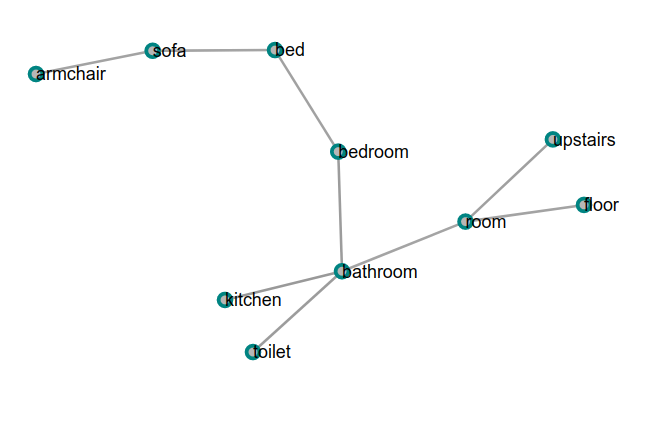
\includegraphics[width=.4\linewidth]{cluster_16}
  }
  \subfloat[]{
    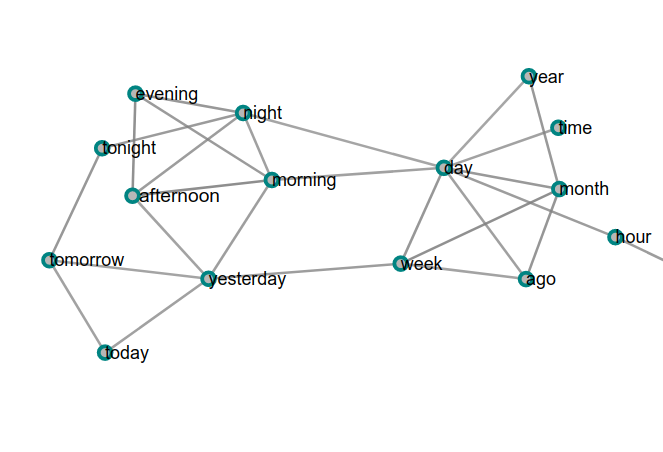
\includegraphics[width=.4\linewidth]{cluster_15}
  }
  \hspace{0mm}
   \subfloat[]{
    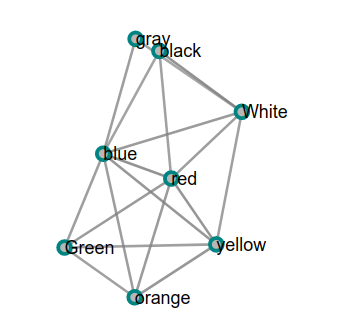
\includegraphics[width=.4\linewidth]{cluster_13}
  }
  \subfloat[]{
    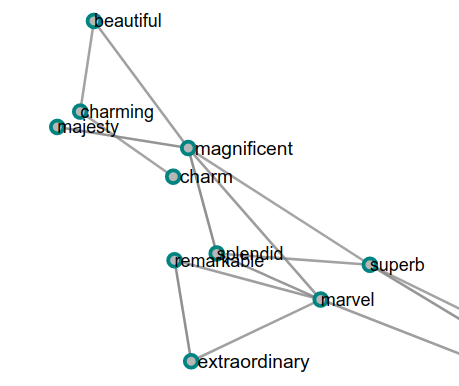
\includegraphics[width=.4\linewidth]{cluster_12}
  }
  \hspace{0mm}
   \subfloat[]{
    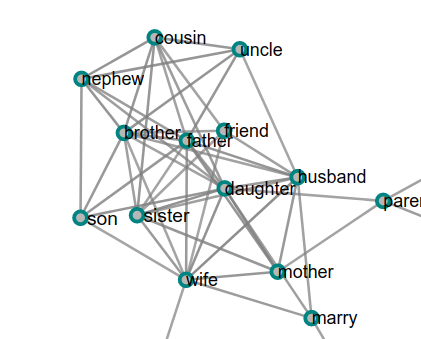
\includegraphics[width=.4\linewidth]{cluster_6}
  }
  \subfloat[]{
    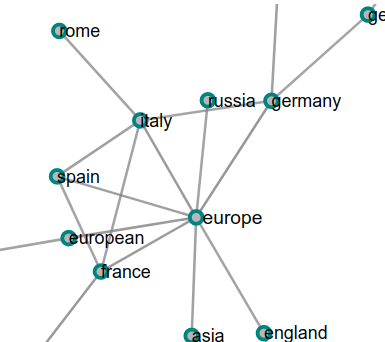
\includegraphics[width=.4\linewidth]{cluster_9}
  }
  \hspace{0mm}
   \subfloat[]{
    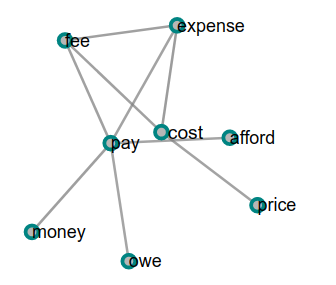
\includegraphics[width=.4\linewidth]{cluster_8}
  }
  \subfloat[]{
    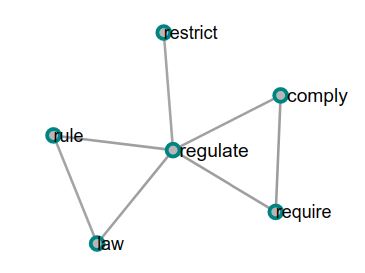
\includegraphics[width=.4\linewidth]{cluster_7}
  }
  \caption{Clusters formed at a threshold of similarity score greater than 0.7}
  \label{fig:clusters}
\end{figure*}

\section{Future Work}
The system has a limitation on operating on the words that do not have a learned representation on the vector space. Which could be rectified by learning a custom word vector specific to the domain. This feature could create a new use case like a tool to learn jargon specifics to a new domain.

The current design of the application is to learn by practice. The sessions can be redesigned to teach new words. Another aspect of extending this work would be to add more learning activities and evaluating their impact on learning.

On the user interface, a mobile application can be used to attract learners. The number of activity types is limited for now, but future work can be an implementation of other activity types. Currently, this system is one learner limited, but after implementation of the login screen and maintaining the database of learners with sessions can also be a helpful feature. Use of text to speech can improve learner's pronunciation. 

Accounting for the forget-factor, the amount of knowledge learner lose with the period of inactivity could be another interesting extension.  Extending as a tool to acquire the pre-requisites: Like acquiring commonly used proper nouns specific to a place before going to the place; Getting introduced to nouns and verbs specific to a novel or tv series.


% include your own bib file like this:
\bibliography{vocabby}
\bibliographystyle{vocabby_natbib}
\end{document}
